\documentclass[11pt]{article}
% /usr/local/texlive/2013/bin/x86_64-darwin/pdflatex 
\usepackage[T1]{fontenc}
\usepackage[utf8]{inputenc}
\usepackage[fleqn]{amsmath}
\usepackage{amssymb}
\usepackage{graphicx}
\usepackage{hyperref}
\usepackage{parskip}
\usepackage{tikz} 
\usepackage{wrapfig} 
\usepackage{alltt}

\renewcommand{\ttdefault}{txtt}

\usepackage[letterpaper]{geometry}
\linespread{1.5}
\usepackage[font=small,labelfont=bf]{caption}
%\usepackage{cancel}

% körper und mengen
\newcommand{\setn}{\mathbb N}
\newcommand{\setr}{\mathbb R}
\newcommand{\setc}{\mathbb C}
\newcommand{\setk}{\mathbb K}

% reihe von #1 bis unendlich über #2
\newcommand{\reihe}[2]{\sum\limits_{#1}^{\infty}{#2}}
% summe von #1 bis #2 über #3
\newcommand{\summe}[3]{\sum\limits_{#1}^{#2}{#3}}
% integral von #1 bis #2 über #3 nach #4
\newcommand{\integrald}[4]{\int\limits_{#1}^{#2}{#3 \; \mathrm d#4}}
% integral von #1 bis #2 über #3 (d/dx muss dann selbst angegeben werden)
\newcommand{\integral}[3]{\int\limits_{#1}^{#2}{#3}}
% integralberechnung von #1 bis #2 über 3
\newcommand{\integralv}[3]{\left[ #3 \right]_{#1}^{#2}}
% betrag mit wachsenden betragsstrichen
\newcommand{\betrag}[1]{\left| #1 \right|}
% limes n gegen unendlich
\newcommand{\limesn}[1]{\lim\limits_{n \to \infty}{#1}}
% limes h gegen 0
\newcommand{\limesh}[1]{\lim\limits_{h \to 0}{#1}}
% vektor kurzschreibweise...
\newcommand{\vect}[1]{\left(\begin{array}{c}#1\end{array}\right)}
%normen
\newcommand{\norm}[1]{\left \Vert {#1} \right \Vert}
\newcommand{\normzwei}[1]{\norm {#1}_{2}}
\newcommand{\norminfty}[1]{\norm {#1}_{\infty}}
\newcommand{\qed}{\hfill \ensuremath{\Box}}
% namentabelle till lukas stefan
\newcommand{\lukas}{\begin{center}
	\begin{tabular}{c|c}
		Name & Student ID \\
		\hline
		Lukas Pfahler & 577332 \\
	\end{tabular}
\end{center}}
% gruppe
\newcommand{\gruppe}[1]{\begin{center} Gruppe {#1} \end{center}}

\title{Information Retrieval and Web Search - Project Phase 2}
\author{Lukas Pfahler \and Tejas Umakanth}
\begin{document}
\maketitle
\section{Collaboration Details}	
	Lukas implemented the web interface, the Lucene search engine backend and the Hadoop backend including the ranking algorithm used for Hadoop search as well as a MapReduce Job for reading aggregated JSON Input, creating a inverted index and outputting it in JSON files. Tejas worked on a MapReduce job to create a inverted index and used his implementation to compare the performance with Lucene indexing.
\section{Architecture}
	\subsection{Indexing}
		Our crawler stored each document in a separate JSON file named \texttt{\{id\}.json}. These files are roughly 8kb each, so we had to merge files into bigger files in order to process them with Hadoop efficiently. We create new, bigger JSON files by concatenating the objects from the small JSON files in a list, until we reach a file size of more than 10mb.

		We wrote a custom \texttt{FileInputFormat} subclass for loading and parsing these aggregated JSON files. Like with our Lucene indexing strategy, we for each image extract the caption as well as all the comments and use this text data for indexing. We remove some stopwords as well as all punctuation (including hashtags). We noticed, that many captions are merely a list of hashtags and not a real text in the traditional IR sense. Thus our Hadoop Index doesn't index hashtags separately. Our FileInputFormat outputs key value pairs \texttt{({Text~=>Text})}, where the key is the document id and the text is all extracted data.

		Our MapReduce Job for creating an inverted index is pretty basic: The Mapper takes a pair $(id \mapsto doc)$ and for  each $word \in doc$ maps $(word \mapsto id)$.

		The Reducer then gets a list of document ids for one word and combines these document ids to a map from document ids to counts: $$\{(word \mapsto id_i)\} \xrightarrow{reduce} \left\{\left(word \mapsto \{(id_i,\#wordCount)\}\right)\right\}$$%\texttt{reduce :: [Text] => (Text => IntWritable)}.

		The maps the Reducer produces are then written to JSON index files using our custom \texttt{FileOutputFormat} subclass. We considered writing all words to a single JSON index, which was inefficient for looking up a single word. Then we considered writing each word to a separate JSON index file, which is very inefficient in the Hadoop Job, because of the small file sizes. We decided on a solution in the middle; we create 1024 index files and decide which word to write to which file using a hash function. We understand that using a fixed number of files is a bad idea in terms of scalability, but decided for this technique because of its simplicity and because for our fixed-sized dataset it is very efficient, since we don't need additional index structures. 

		The index file has the following form:
		\begin{alltt}
		\{
		    "word1" : \{
		        "documentCount" : 2,
		        "documents": [
		            \{
			            "document" : "id1",
			            "score" : 1.0
		            \},
		            \{
			            "document" : "id2",
		                "score" : 2.0
		            \},
		            ...
		        ]
		    \},
		    "word2" : \{...\},
		    ...
		\}
		\end{alltt}

	\subsection{Webinterface and Search Engine}
		\begin{figure}[h]
			\begin{center}
				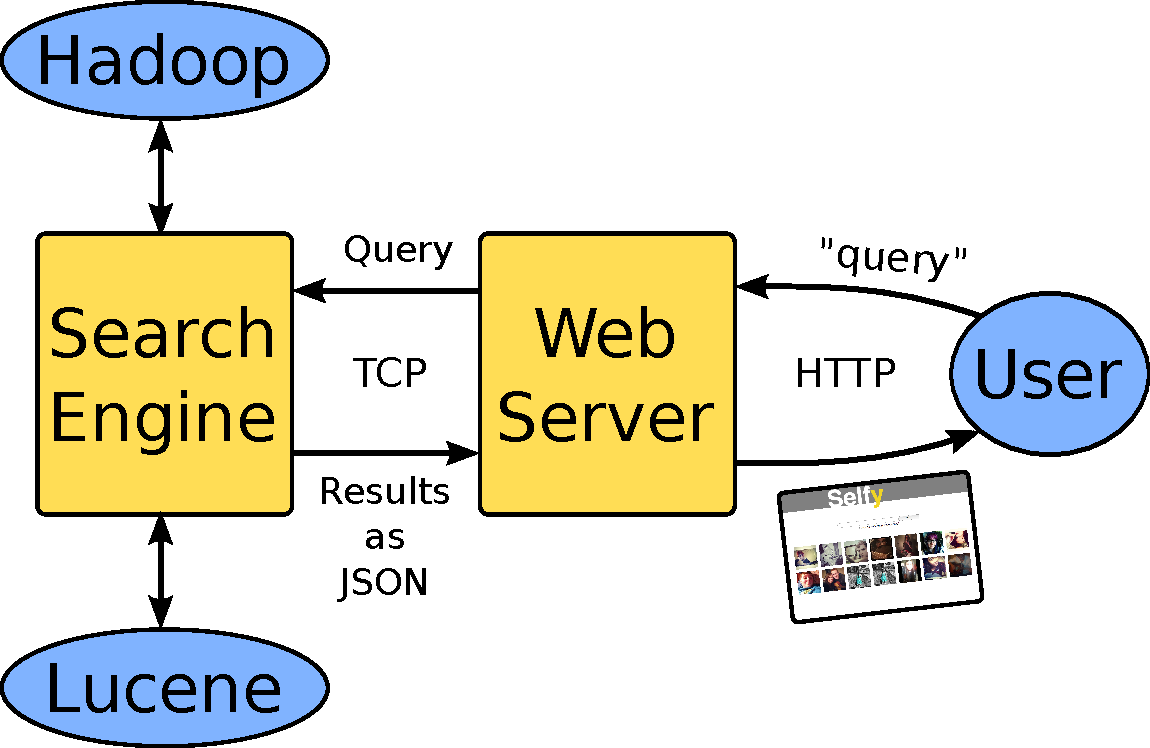
\includegraphics[width=0.9\textwidth,keepaspectratio]{architecture.pdf}
			\end{center}
			\caption{An overview of our search engine architecture.}
			\label{fig1}
		\end{figure}

		The actual search engine and the web interface are two separate components; the web server is written based on node.js and the search engine is written in Java, they exchange information using a TCP connection, as seen in figure~\ref{fig1}.

		The search engine listens for connections on port 8999. To search, a client connects and writes 'x query', where $x$ is either 'l' for Lucene or 'h' for Hadoop and query is the search query. Our search engine then performs the search using either our index created by Hadoop or our index created by Lucene. The results are returned in JSON format.

		The Lucene search uses the default Lucene ranking algorithm. Our Lucene index indexed hashtags separately, thus each term $\#$\texttt{term} in a query is replaced with \texttt{hashtags:term} to tell Lucene to look it up in the right index.

		For Hadoop-based search, we lookup each term of the query in the right index file by applying the hash function and parsing the right JSON file. This way we can retrieve a list of documents with word counts. For each query we maintain a map from document to score, containing all the documents retrieved for any term of the query. For the scoring function we use a simplified BM25.

		For the web interface we decided to go with node.js again. We start a http server on port 8080 and wait for requests. Once a user enters a query, our webserver opens a TCP connection to our search engine backend, specifying whether to use Lucene or Hadoop and relaying the query. The backend executes the query and returns the results as JSON. The results are then output to the user by the web server as a grid of thumbnail images. Additional information like the caption and the comments for each image is loaded in an asynchronous fashion using AJAX and JSON when the user requests it by clicking on an image.



\section{Usage}
	\subsection{Indexer}
		To run the indexer execute the following command:
		\begin{alltt}
			sh indexer.sh \{dataDir\}
		\end{alltt}	
		where \texttt{\{dataDir\}} contains the aggregated JSON files.
		This will create a directory \texttt{HadoopIndex} with 1024 JSON index files.
	\subsection{Web Server}	
		To start the web server on port 8080 execute the following command:
		\begin{alltt}
			sh server.sh \{dataDir\} \{hadoopDir\} \{luceneDir\}
		\end{alltt}	
		where \texttt{\{dataDir\}} contains the raw crawled data, \texttt{\{hadoopDir\}} contains the hadoop index and \texttt{\{luceneDir\}} contains the lucene index.

		To shutdown the server properly, search for 'killtheserver'.
\section{Performance}
	Tejas Part...
\section{Screenshots}
	\begin{figure}[H]
		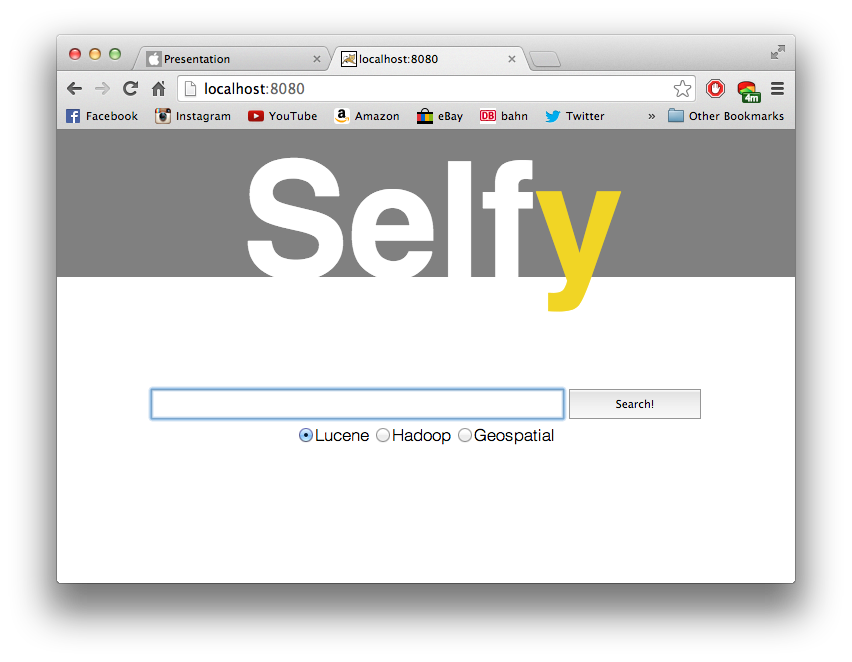
\includegraphics[keepaspectratio,width=\textwidth]{screenshot1.png}
		\caption{The search front page}
	\end{figure}
	\begin{figure}[H]
		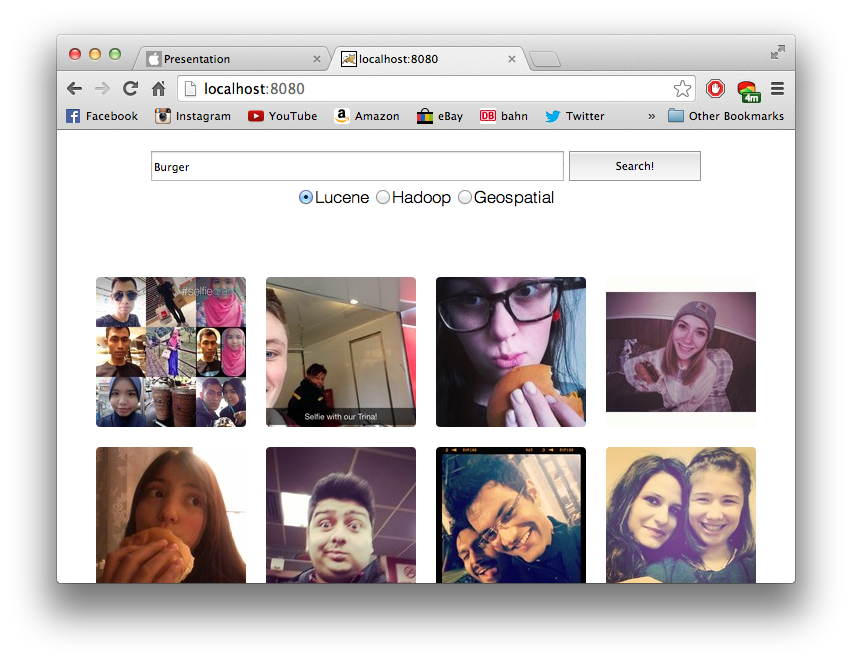
\includegraphics[keepaspectratio,width=\textwidth]{screenshot2.png}
		\caption{The results}
	\end{figure}
	\begin{figure}[H]
		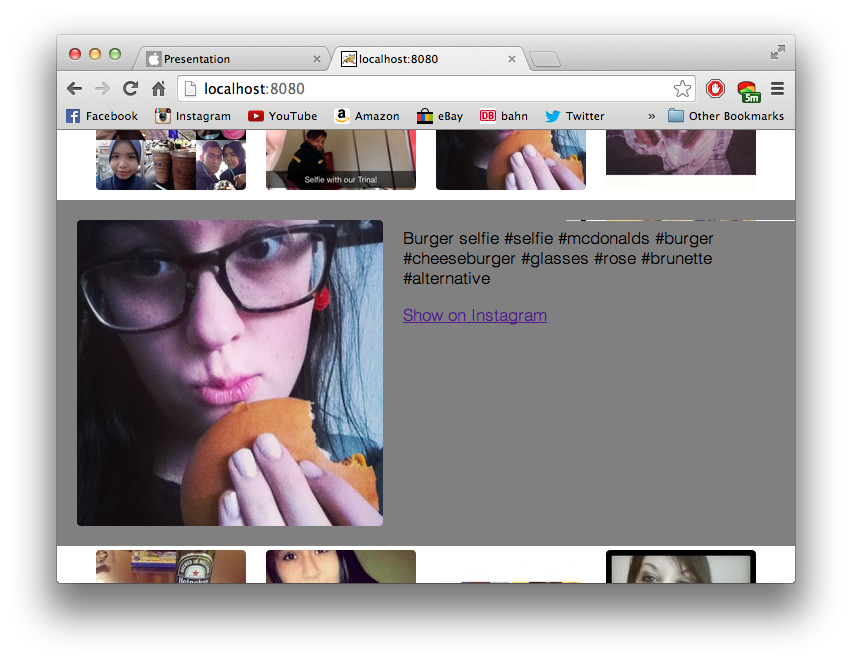
\includegraphics[keepaspectratio,width=\textwidth]{screenshot3.png}
		\caption{More details on one document}
	\end{figure}
\end{document}
